\documentclass[letterpaper, 11pt]{article}

\usepackage[top=0in, bottom=1in, left=1in, right=1in, includehead, includefoot]{geometry}
\usepackage[utf8]{inputenc}
\usepackage[english,russian]{babel}
\usepackage{titlesec}
\usepackage{xcolor}
\usepackage{graphicx}
\usepackage{wrapfig}
\usepackage{float}
\usepackage{hyperref}
\usepackage{amssymb}



\definecolor{headerColor}{HTML}{003300}
\renewcommand{\familydefault}{phv}

\titleformat{\section}[hang]
    {\Large}
    {\thesection}
    {0.3in}
    {}
    [\color{headerColor}\hrule height 0.5pt]



\begin{document}

    \begin{wrapfigure}{R}{0.25\textwidth}
        \centering
        \vspace{-5pt}
        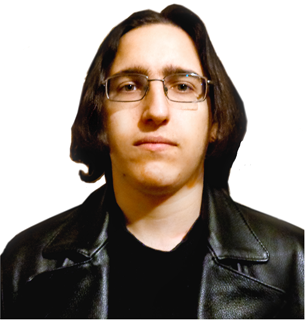
\includegraphics[width=0.25\textwidth]{src/images/pho_small_cut.png}
    \end{wrapfigure}

    \noindent
    \Huge
    Danila Kiver \\
    \normalsize

    \noindent
    Location: Moscow, Russia. \\

    \noindent
    Contacts: danila.kiver@mail.ru or +7-909-645-38-84. \\

    \noindent
    Education: B. Sc. (Moscow State University, Faculty of Physics, Chair of Computer Methods of Physics). \\

    \noindent
    Communication: upper-intermediate English; experience with completely distributed teams (including english-speaking ones). \\

    \noindent
    Public profiles (clickable links): \href{https://stackoverflow.com/users/7191047/danila-kiver}{StackOverflow}, \href{https://unix.stackexchange.com/users/297621/danila-kiver}{Unix StackExchange}, \href{https://github.com/QazerLab}{GitHub}.





    \section{Experience}

    5 years summary.

    \begin{itemize}
        \item
            Senior Software Engineer \\
            \footnotesize
                EPAM Systems, May 2018 -- Dec 2019
            \normalsize
            
            \begin{itemize}
                \item
                    EPAM PERF project: migrated the solution into the cloud (Ubuntu Server bare--metal machines $\rightarrow$ GKE); was involved both in infrastructure and development teams.
                \item
                    Axway Syncplicity project (\url{https://www.syncplicity.com}): developed and supported system backend (message queue, content search, cloud storage) and on-premises services (on-prem storage connector). The team was english-speaking (including native American speakers). Tech stack: SpringBoot Java-services + MariaDB; underlying infrastructure --- CentOS 7 VMs in AWS EC2. Some legacy services were also written in Scala + Play.
                \item
                    Participated in internal mentoring program for developers (as a mentor).
                \item
                    Participated in internal and external technical meetups as a speaker (topic --- internals of Linux containers and underlying technologies).
            \end{itemize}

        \item
            Senior Software Engineer \\
            \footnotesize
                NetCracker Technology, Apr 2017 -- May 2018
            \normalsize
            
            \begin{itemize}
                \item
                    Developed Zero Touch Provisioning system prototype for SD-WAN project. Tech stack: SpringBoot Java-services + PostgreSQL; underlying infrastructure --- OpenShift Origin on CentOS 7 VMs in OpenStack (private cloud).
                \item
                    Developed and supported HA PostgreSQL cluster distribution. HA was achieved by using Patroni framework.
            \end{itemize}

        \item
            Software Engineer \\
            \footnotesize
                NetCracker Technology, Nov 2014 -- Mar 2017
            \normalsize

            \begin{itemize}
                \item
                    Migrated existing monolithic solution (WildFly + Spring + PostgreSQL) to the cloud environment (OpenShift Origin).
                \item
                    Participated in development and support of HA infrastructure based on Pacemaker.
                \item
                    Developed and supported low-level Java libraries of internal platform (persistence, history, platform abstraction).
            \end{itemize}
    \end{itemize}





    \section{Sanity Check}

    \renewcommand{\labelitemi}{\checkmark}

    The development culture is a keystone for keeping the project maintainable disregarding what tools the team uses and how skillfull the team is. Without proper development culture any project becomes an unmaintainable mess as soon as possible. The checklist below proves that I follow well-known development best practices and expect the team to follow them as well:

    \begin{itemize}
        \item I respect Twelve-Factor App principles and follow them.
        \item I understand the importance of branching and versioning. I tend to use SemVer and Trunk-based flow, but understand that the team may adhere to other versioning and branching schemes. In any case, branching and versioning strategies must be explicitly documented and justified.
        \item I understand the importance of the code review. I understand that high-quality review is possible only for small change sets with detailed merge request descriptions and commit messages, explaining the main idea and the reason of the change set.
        \item I understand that CI/CD is an approach to the development and delivery organization rather than just specific tools and their presence in the toolchain. Using tools like Jenkins Pipeline and Artifactory does not automatically mean having CI/CD.
        \item I understand that DevOps is a development culture and methodology rather than the name of a standalone team of automation engineers / network engineers / release engineers / ... (place your DevOps anti-pattern here).
        \item I understand that the items above are the reasons why CI/CD and DevOps are impossible without the proper mindset of the development team and without understanding of the underlying infrastructure and development processes by developers.
    \end{itemize}
    
    \renewcommand{\labelitemi}{\textbullet}





    \section{Technical Skills}

    \begin{itemize}
        \item Linux (overall experience, including desktop --- 10+ years with different distros; industrial experience with servers --- 5 years with CentOS 6/7 and Ubuntu Server).
        \item Languages: Java 8 (main language), bash.
        \item Infrastructure: Docker, OpenShift Origin up to 3.6 (including the cluster administration) and Kubernetes, IaaS --- OpenStack and AWS (as a user); minor experience with Google Cloud.
        \item SCM: Ansible, Salt.
    \end{itemize}





    \section{Professional Interests}

    Learning alternative (to my current tech stack) development approaches and paradigms (Rust, Haskell, C). Diving deep into technologies I use (Docker, Linux kernel, JDK/JVM, etc.; reading the code, experimenting and breaking everything I can break). \\

    \noindent
    Trying to solve some interesting problems at StackOverflow and Unix StackExchange (links to the profiles are in the header). When required, perform minor improvements and fixes in open-source projects.

\end{document}
